\documentclass[border=5mm]{standalone}
\usepackage{tikz}
\begin{document}
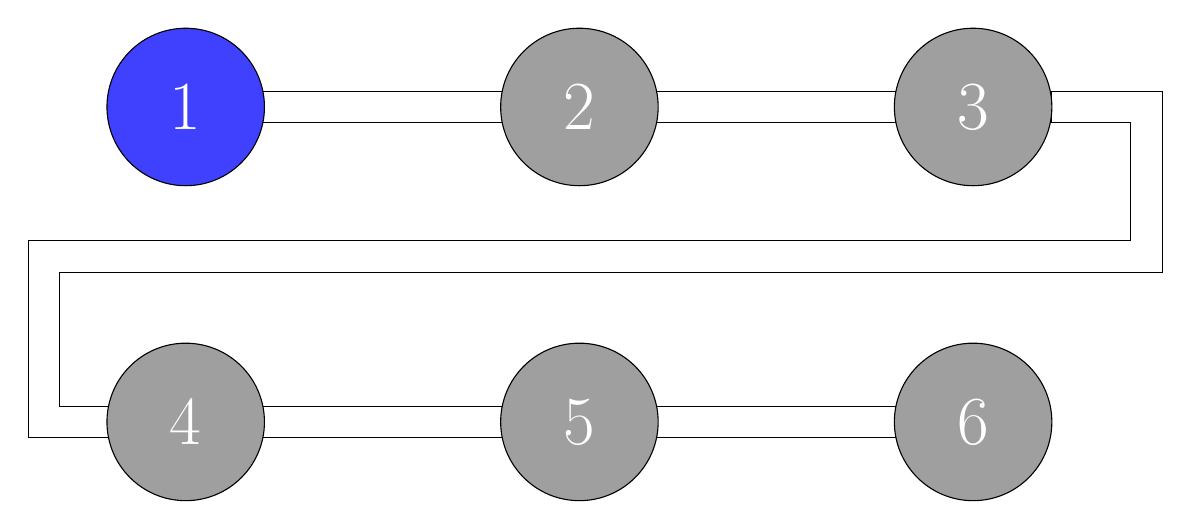
\begin{tikzpicture}
    \draw (0, -0.2) rectangle (5, 0.2);
    \draw (5, -0.2) rectangle (10, 0.2);
    \draw (0, -4.2) rectangle (5, -3.8);
    \draw (5, -4.2) rectangle (10, -3.8);
    \draw (11, -0.2) -- (12, -0.2) -- (12, -1.7) -- (-2, -1.7) -- (-2, -4.2) -- (0, -4.2) -- (0, -3.8) -- (-1.6, -3.8) -- (-1.6, -2.1) -- (12.4, -2.1) -- (12.4, 0.2) -- (11, 0.2) --(11, -0.2);
    \draw [fill=blue!75, text=white] (0, 0) circle (1) node {\Huge$1$};
    \draw [fill=gray!75, text=white] (5, 0) circle (1) node {\Huge$2$};
    \draw [fill=gray!75, text=white] (10, 0) circle (1) node {\Huge$3$};
    \draw [fill=gray!75, text=white] (0, -4) circle (1) node {\Huge$4$};
    \draw [fill=gray!75, text=white] (5, -4) circle (1) node {\Huge$5$};
    \draw [fill=gray!75, text=white] (10, -4) circle (1) node {\Huge$6$};
\end{tikzpicture}
\end{document}